%%%%%%%%%%%%%%%%%%%%%%%%%%%%%%%%%%%%%%%%%
% Short Sectioned Assignment
% LaTeX Template
% Version 1.0 (5/5/12)
%
% This template has been downloaded from:
% http://www.LaTeXTemplates.com
%
% Original author:
% Frits Wenneker (http://www.howtotex.com)
%
% License:
% CC BY-NC-SA 3.0 (http://creativecommons.org/licenses/by-nc-sa/3.0/)
%
%%%%%%%%%%%%%%%%%%%%%%%%%%%%%%%%%%%%%%%%%

%----------------------------------------------------------------------------------------
%	PACKAGES AND OTHER DOCUMENT CONFIGURATIONS
%----------------------------------------------------------------------------------------

\documentclass[paper=a4, fontsize=11pt]{scrartcl} % A4 paper and 11pt font size

\usepackage[T1]{fontenc} % Use 8-bit encoding that has 256 glyphs
%\usepackage{fourier} % Use the Adobe Utopia font for the document - comment this line to return to the LaTeX default
\usepackage[english]{babel} % English language/hyphenation
\usepackage[utf8]{inputenc}  %allows non-English characters
\usepackage{amsmath,amsfonts,amsthm} % Math packages
\usepackage{float}

\usepackage{sectsty} % Allows customizing section commands
%\allsectionsfont{\centering \normalfont\scshape} % Make all sections centered, the default font and small caps
\allsectionsfont{\centering}

\usepackage{fancyhdr} % Custom headers and footers
\pagestyle{fancyplain} % Makes all pages in the document conform to the custom headers and footers
\fancyhead{} % No page header - if you want one, create it in the same way as the footers below
\fancyfoot[L]{} % Empty left footer
\fancyfoot[C]{} % Empty center footer
\fancyfoot[R]{\thepage} % Page numbering for right footer
\renewcommand{\headrulewidth}{0pt} % Remove header underlines
\renewcommand{\footrulewidth}{0pt} % Remove footer underlines
\setlength{\headheight}{13.6pt} % Customize the height of the header

%\usepackage{geometry}
%\usepackage{pdflscape}


%\numberwithin{equation}{section} % Number equations within sections (i.e. 1.1, 1.2, 2.1, 2.2 instead of 1, 2, 3, 4)
%\numberwithin{figure}{section} % Number figures within sections (i.e. 1.1, 1.2, 2.1, 2.2 instead of 1, 2, 3, 4)
%\numberwithin{table}{section} % Number tables within sections (i.e. 1.1, 1.2, 2.1, 2.2 instead of 1, 2, 3, 4)

%\setlength\parindent{0pt} % Removes all indentation from paragraphs - comment this line for an assignment with lots of text

\usepackage{caption}
%\usepackage{topcapt}

\usepackage{booktabs}

\usepackage{graphicx}
\usepackage{adjustbox}


%shortcuts for typing variance and expectation
\newcommand{\E}{\mathrm{E}}
\newcommand{\Var}{\mathrm{Var}}
\newcommand{\RR}{{\mathbb R}}

\theoremstyle{definition}
\newtheorem{prob}{Problem}

\usepackage{listings}
\usepackage{hyperref}

%----------------------------------------------------------------------------------------
%	TITLE SECTION
%----------------------------------------------------------------------------------------

\newcommand{\horrule}[1]{\rule{\linewidth}{#1}} % Create horizontal rule command with 1 argument of height

\title{
\normalfont \normalsize
\textsc{UPC - Discrete and algorithmic geometry} \\ [25pt] % Your university, school and/or department name(s)
\horrule{0.5pt} \\[0.4cm] % Thin top horizontal rule
\huge Exam project: Enumerate all neighborly $4$-polytopes on $8$ vertices \\ % The assignment title
\horrule{2pt} \\[0.5cm] % Thick bottom horizontal rule
}

\author{Alba Delgado \and Petar Hlad \and Rebecca Guardado \and Simon Van den Eynde} % Your name

\date{\normalsize\today} % Today's date or a custom date

\begin{document}


\maketitle % Print the title


%----------------------------------------------------------------------------------------
%	INTRO
%----------------------------------------------------------------------------------------

\section{Introduction}
%Write here what will do 
Our goal is to solve the following problem:
\begin{prob}
Enumerate all simplicial neighbourly 4-polytopes on 8 vertices up to combinatorial equivalence.
\end{prob}
The idea of how we will solve this problem is the following. We start from all possible affine Gale diagrams of a 4-polytope on 8 vertices. These are point configurations of 8 points in the plane, each with an assigned positive or negative sign. We check which of these affine Gale diagrams correspond to neighbourly, simplicial polytopes, and consider only these configurations. Then, check whether they correspond to the same polytope (i.e. to a combinatorially equivalent polytope) and once we have all different Gale diagrams, retrieve the polytope they correspond to.


%%%%%%%%%%%%%%%%%%%%%%%%%%%%%%%%%%%%%%%%%%%%%%%%%%%%%%%%%%%%%%%%
\section{Results}
%Write here what the result is
In figure~\ref{fig:gale} we show all neighbourly Gale diagrams we found.
\begin{figure}[!htb]
\centering
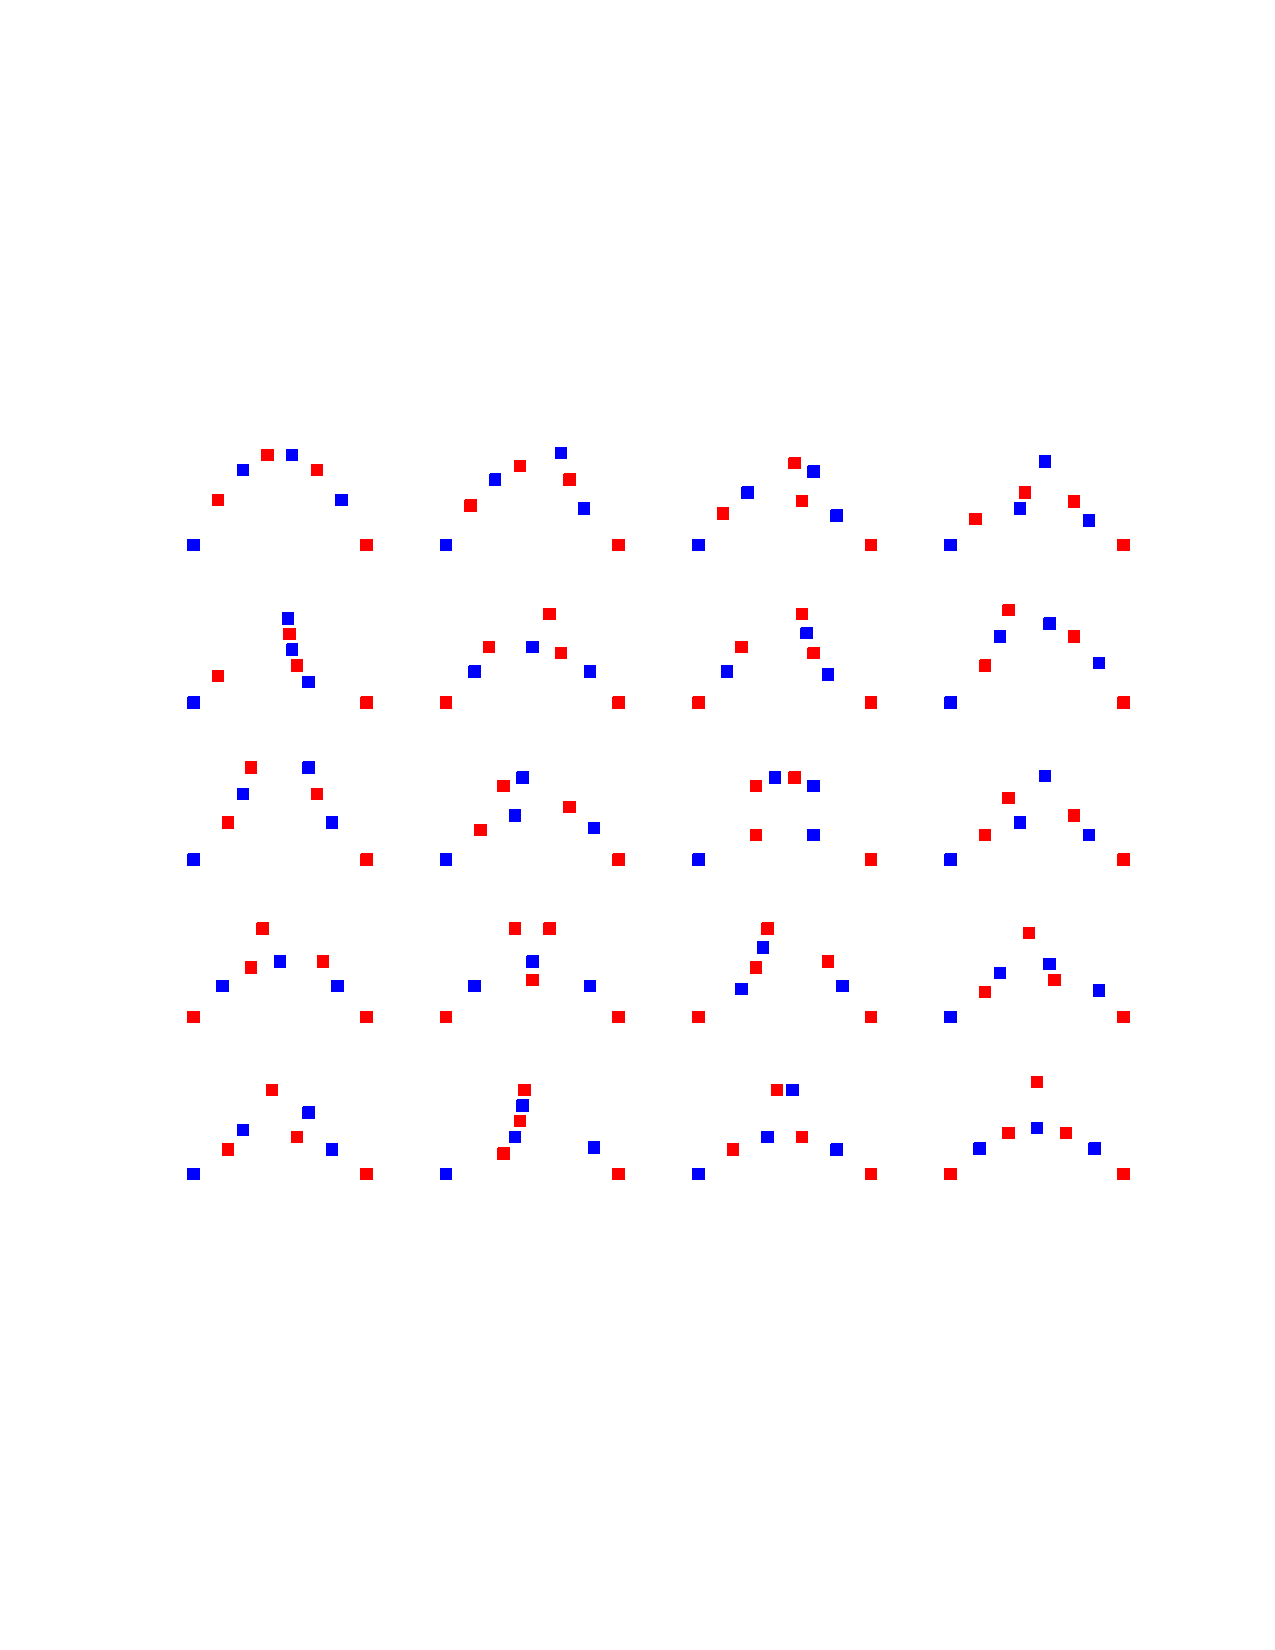
\includegraphics[trim={0 5cm 0 5cm},clip,width=\textwidth]{gale_diagrams.pdf}
\caption{All neighbourly Gale Diagrams, some isomorphic.}
\label{fig:gale}
\end{figure}


After filtering on isomorphisms, we found $3$ isomorphism classes. For each of these classes we give the coordinates of $1$ polytope in figure~\ref{fig:polyPoints}. These are $3$ different neighbourly simplicial $4$-polytopes on $8$ vertices up to combinatorial equivalence.

\begin{figure}[!htb]
\lstinputlisting{polytopes.txt}
\caption{The coordinates for all $3$ different neighbourly $4$-polytopes on $8$ vertices up to combinatorial equivalence}
\label{fig:polyPoints}
\end{figure}


%%%%%%%%%%%%%%%%%%%%%%%%%%%%%%%%%%%%%%%%%%%%%%%%%%%%%%%%%%%%%%%%
\section{Discussion}
%Discuss the result here, say why it is special, if it is (un)expected?
Since this is a studied problem (see \cite{GrSr67}), we know that the 3 different simplicial neighbourly 4-polytopes on 8 vertices are $C_4(8)$, $N_8$ and $N_8^*$, where $C_4(8)$ is the cyclic polytope on 8 vertices, and an explicit description of $N_8$ and $N_8^*$ can be found in page 125 of \cite{Gr03}.


%%%%%%%%%%%%%%%%%%%%%%%%%%%%%%%%%%%%%%%%%%%%%%%%%%%%%%%%%%%%%%%%
\section{Programming details}
%Describe any non-trivial things you programmed, or where you encountered a lot of trouble.
The first thing the code does is find a finite number of points in the plane where our points of the different Gale diagrams will be. To do this, we use the fact that not the exact the location of the points is important, but the position of each point with respect to the lines defined by the other points. Therefore we can fix two of our points, $1$ and $2$, to be the lowermost, and choose the lines through these two points on which the other points will lie. To get more or less reasonable coordinates, we chose to fix the points $(0,0)$ and $(2,0)$, and the lines through them and $(1,i)$, with $i =1,\ldots,6$. Then, the points that we will consider to be on the Gale diagram are the intersections through the lines from $1$ and from $2$.\\
\\
\texttt{enumerate\underline{ }all\underline{ }gale} uses backtracking to find all possible combinations of  points on the grid of intersections previously defined. To do this, it takes into account that for a polytope to be simplicial, no three points can be aligned, so when it chooses a point to lie in a line through 1, it of course lies in a line through 2 and automatically bans any other point to go through the same line through 2. This procedure produces $6! = 720$ configurations of points in the plane. In addition, it has to give a sign to each point. The first sign is prescribed (since configurations with all signs interchanged are equivalent, we can prescribe one sign). Furthermore, only configurations with $3$ or $4$ negative signs are considered, since other configurations will not result in a neighbourly polytope. This gives for each of the Gale diagrams found $7\choose 5$ $+$ $7\choose 4$ $= 91$ possible combinations of signs, so in total our program runs initially through $720\cdot 91 = 65520$ possible Gale diagrams.\\
\\
Since the computation of checking if a Gale diagram is neighbourly is a bit expensive, we try to reduce the number of Gale diagrams by eliminating the ones that are not simplicial. \texttt{isSimplicial} checks that in every set of four points of the diagram, no three points are aligned. After this step we are left with 51688 Gale diagrams.\\
\\
\texttt{is\underline{ }neighborly} loops through every pair of two points, and for each choice of pair, it removes the pair from the Gale diagram and then checks if the convex hulls of the negative and positive points intersect. After this step we are left with 20 Gale diagrams that can be seen in \ref{fig:gale} .\\
\\
\texttt{makeVertexFacetStructure} gives the vertex-facet lattice obtained from the Gale diagram, by creating a vertex $i$ for every point $i$ $(i=0,\ldots,7)$ and making a vertex for every facet, so we have $28$ vertices. The result is returned in an igraph\underline{ }t object, from the igraph library\footnote{\url{http://igraph.org/c/}}. \\
\\
To check whether two Gale diagrams are isomorphic, we use the in igraph built in graph isomorphism algorithm (uses BLISS). We find 3 different combinatorial types. Of the 20 Gale diagrams shown in \ref{fig:gale}, 7 represent one polytope, 8 another and 5 another.\\
\\
\texttt{gale\underline{ }to\underline{ }polytope} takes an affine Gale diagram that we know corresponds to a simplicial and neighbourly polytope and returns projective coordinates for the vertices of the polytope. The procedure follows the reverse idea of how the vectors of the Gale transform are obtained. We initially have a matrix $B$ with the Gale points in the plane, and a sign assigned to each of the points. We project from the origin in $\RR^3$ all positive points to the plane $Z = 1$, and all negative points to the plane $Z = -1$. Once we have this, we need the vector configuration to be balanced. Therefore we scale the vectors. We need coefficients $\lambda_i$ that multiply each vector $v_i$ and such that then all rows of the matrix $B$ sum to zero. To do this we can fix $5$ of the $\lambda_i$ since any other set of three points will have full rank because we are taking Gale diagrams where no three points are aligned, and then we only need to solve a $3x3$ linear system of equations. After the rescaling of the vectors of the Gale transform, we can get the kernel of their matrix and the vector of all ones is in its affine span, so we either move it or add it to the last row (which we can do by Steinitz Exchange Lemma) and we get 8 points of $\RR^4$ in projective coordinates that are the vertices of a polytope to which the Gale diagram corresponds to.\\
\\
\section{Proof}
%Describe why the program gives the correct result, use theorems and proof them or refer to the proof in a paper/book.
There are some non-trivial results used to solve this problem that are worth discussing.\\
\\
The theory of Gale diagrams and why they allow us to reconstruct polytopes can be found in \cite{Ma02} and \cite{Zi93}. We claim that  only the position of a point in the diagram relative to the position of the lines defined by other points is important, as opposed to the exact coordinates of the point. That is quite clear: we select a point, and we can read from the diagram the faces of the polytope. This is done by looking at intersections of the convex hulls of negative and positive sets of points, and in a set where our selected point participates, it is clear that if the intersection is empty this does not change unless our point crosses a line of opposite sign, and if it is not empty this cannot change unless it crosses a line of opposite sign. \\
\\
To check whether two polytopes are combinatorially equivalent, we check the isomorphism of the vertex-facet lattice, instead of the face lattice. The vertex-facet lattice is enough to determine the combinatorial type of a polytope because the face lattice is graded, atomic and coatomic (\cite{Ma02}).\\
To make sure our program doesn't make any rounding errors, we used rational numbers from the GMP-library.
\\
Finally, our construction of a polytope from a Gale diagram is based on linear algebra. It is simply reversing the construction of a Gale diagram.

\begin{thebibliography}{9}
\bibitem{Gr03}
B. Gr{\"u}nbaum, Convex polytopes. \textit{Graduate
Texts in Mathematics} vol 221, (2003).
\bibitem{GrSr67}
B. Gr{\"u}nbaum, V.P. Sreedharan, An enumeration of simplicial 4-polytopes with 8 vertices. \textit{Journal of Combinatiorial Theory 2}, 437-465, (1967).
\bibitem{Ma02}
J. Matou{\v s}ek, Lectures on Discrete Geometry. \textit{Graduate
Texts in Mathematics} vol 212, (2002).
\bibitem{Zi93}
G. Ziegler, Lectures on Polytopes. \textit{Graduate
Texts in Mathematics} vol 212, (1993).
\end{thebibliography}
\end{document}